\section{Revisão literária}

Serão apresentados na presente seção alguns pontos que, segundo a literatura, nortearão o estudo estatístico do trabalho em questão, abordando alguns pontos importantes para realização do planejamento e análise dos experimentos. Logo em seguida, serão aplicados os conceitos aqui apresentados.


\subsection{Planejamento e análise de experimentos}

Técnicas de planejamento e análises de experimentos são utilizáveis em empresa, processo de fabricação, desenvolvimento de um novo produto e até em fabricação de commodities. Geralmente a maioria destes processos possuem diversas variáveis controláveis, como temperatura, velocidade, dimensões entre outras. A variação destas variáveis, de modo isolado ou combinado, pode trazer melhorias ou prejuízos a qualidade do produto ou serviço. Com isso, faz-se necessário um estudo analítico de como cada variável pode influenciar o processo \cite{1}. 

O planejamento e análise de experimentos (\textit{Design of Experiments, \textbf{DoE}}) é uma técnica de planejamento de experimentos, ou seja, como os experimentos devem proceder para garantir conclusões assertivas. A validade das conclusões obtidas após análise dos experimentos, são diretamente ligadas ao modo como os experimentos foram realizados, logo, o planejamento do experimento torna-se o ponto mais importante na hora de se analisar algum processo produtivo, bens ou serviços prestados. O planejamento corretamente executado também pode evitar desperdícios, além de isolar e determinar relações das variáveis \cite{1}.

A seguir serão apresentados alguns pontos importantes para análise estatística realizada neste presente trabalho, como: Princípios do planejamento, que irão nortear como deve ser condizido o planejamento de experimentos, bem como etapas para realização dos experimentos e análise dos mesmos \cite{2}.


\subsubsection{Princípios do planejamento de experimentos}

O planejamento de experimentos possui três princípios, que são: Replicação, aleatóriedade e blocagem \cite{2}. 

\subsubsection*{Replicação}

A replicação consiste na obtenção de mais de uma unidade experimental, ou seja, replicar o teste para cada ponto experimental e assim permite que obtenha-se uma estimativa mais precisa, diminuindo a influência de variações indesejadas ou inevitáveis \cite{2}.

\subsubsection*{Aleatoriedade}

Os métodos estatísticos requerem que as observações sejam variáveis aleatórias, de modo a garantir a distribuição igual dos fatores não esperados. Com isso garantem-se estimativas não tendênciosas dos efeitos e erros experimentais, bem como evitar influência sistemática de fatores não controláveis \cite{2}. 
\subsubsection*{Blocagem}

A blocagem é uma técnica extremamente importante, utilizada com o objetivo de aumentar a precisão de um experimento. Este princípio pode ser aplicado em alguns casos onde deseja-se isolar algum fator conhecido, analisando de forma individual sua influência sobre o processo. A mudança de pessoas no processo experimental ou a mudança de lote de um produto pode ser visto a princípio como um fator não desejado de ser analisado, logo, o princípio de blocagem permite que o mesmo seja isolado, porém, não ignorado\cite{2}. 

\subsubsection{Etapas para o desenvolvimento de experimentos}
\label{subsec:etapas}

Coleman e Montgomery (1993) propõem as seguintes etapas para o desenvolvimento de um planejamento de experimentos \cite{3}:

\begin{enumerate}
    \item \textbf{Caracterização do problema:}
    A definição do problema que está sendo analisado é uma etapa essencial para se entender o estudo analítico. Para isso se faz necessário conhecimento sobre todo o processo para assim definir de forma clara o objetivo e relatar de forma específica o problema analisado.

    \item \textbf{Escolha dos fatores de influência e níveis:}
    Para conduzir o experimento deve-se escolher os fatores variáveis, os intervalos sobre os quais esses fatores variarão e os níveis específicos. Para tanto é necessário conhecimento do processo, experiências práticas e teóricas para determinar tais fatores mais relevantes para análise experimental.
    \item \textbf{Seleção das variáveis de resposta:}
    É também necessário ao planejar um experimento que se tenha clareza de qual variável-resposta será obtida como parâmetro para qualificar os experimentos. Variável de resposta que não atenda a necessidade do experimento pode levar a conclusões equivocadas. 
    \item \textbf{Determinação de um modelo de planejamento de experimento:}
    A escolha do planejamento envolve consideração sobre o tamanho da amostra (número de replicações) e determinar se há formação de blocos ou outras restrições de aleatorização.
    \item \textbf{Condução do experimento:}
    A condução do experimento deve seguir todo o planejamento, evitando variações de ambiente, métodologia do experimento ou inserção de novas variações não previamente estabelecidas. O responsável pelo experimento e os equipamentos utilizados devem ser mantidos do início ao fim, exceto em casos onde estas variações sejam desejáveis.

    \item \textbf{Análise dos dados:}
    
    Após todas as demais etapas anteriores, os resultados podem ser obtidos com uso de ferramentas e pacotes estatísticos para auxiliar na visualização de gráficos e dados. A verificação da validade do modelo é também um ponto importante para análisar. 

    \item \textbf{Conclusões e recomendações:}
    
    Após a obtenção dos resultados, o experimento deve apresentar conclusões práticas para proporcionar recomendações de ações em cima do processo analisado. As recomendações são frutos das etapas decorridas no planejamento do experimento, ou seja, planejamentos com falhas iram gerar ações equivocadas no processo. 
     
\end{enumerate}

\subsection{Análise de regressão}

Um método muito utilizado nos estudos estatísticos é a análise de regressão. Este método permite examinar a relação entre duas ou mais variáveis que se deseja-se estudar. O método permite por meio de modelos matemáticos avaliar quais as relações entre as variáveis, quais delas são importantes para o processo e quais apresentam pouca relevância \cite{4}. 

As variáveis utilizadas podem ser divididas em duas: Variável Dependente, que é a variável que está sendo estudada, como uma sáida do processo (a influência das demais variáveis será analisada através das variáveis dependentes); e Variável Independente, que são as entradas do estudo, são variáveis que supostamente causam impactos ou certa influência na variável dependente \cite{4}.

A análise de regressão tem por finalidade chegar a algumas conclusões e direcionamentos sobre o processo estudado, as finalidades deste estudo são \cite{4}:

\begin{itemize}
    \item Predição dos dados;
    \item Seleção de variáveis influenciáveis no processo;
    \item Estimação de parâmetros;
    \item Realizar inferências sobre os parâmetros, como: testes de hipóteses e intervalos de confiança.
\end{itemize}

\subsubsection{Tipos de regressão}

A análise de regressão é dividida em alguns tipos, tendo cada uma sua própria especificidade, logo, todo analista de deve saber qual forma usar, variando sua escolha pelo tipo de dado e sua distribuição. Os tipos mais comuns são: Regressão Linear; Regressão Polinomial; Regressão de Poisson; Regressão de Ridge; Regressão Logística e Mínimos quadrados parciais (PLS) \cite{5}. Para fins deste estudo será abordado de forma mais aprofundada a regressão linear. 

\subsubsection*{Regressão linear}

A regressão Linear é um modelo matemático que tem por objetivo observar a relação entre duas ou mais variáveis por meio de uma reta, e utilizar o resultado da função dessa reta para estimar valores e encontrar relações. Quando existe apenas uma variável independente e uma variável dependente, ela é chamada de \textbf{regressão linear simples}. Quando existe mais de uma variável independente, é chamado de \textbf{regressão linear múltipla}. Na equação de regressão linear múltipla, (equação \ref*{eq:regressao}), o 'Y' é a variável dependente, 'X' são as variáveis independentes, $\beta_i$ são os coeficientes de regressão e $\epsilon$ é o termo de erro\cite{5}. 

\begin{equation}
    Y = \beta_1 + \beta_2X_2 + \beta_3X_3 + ... + \beta_iX_i + \epsilon  
    \label{eq:regressao}  
\end{equation}

Como exemplo de uma análise de regressão linear no R (figura \ref*{fig:R}), será analisado os dados a seguir e entender as informações contidas no estudo.
 
\begin{figure}[h]

    \caption{Exemplo de regressão linear no R \cite{5}}
    \centering
    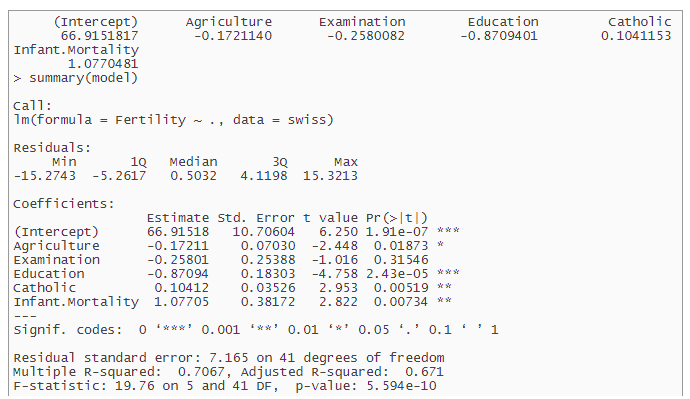
\includegraphics[width=0.8\textwidth]{images/R.png}
    \label{fig:R}
    
\end{figure}

\subsubsection*{R múltiplo}

Esse dado serve para medir a relação linear entre as variáveis dependente e independentes, ou seja, mede o quanto elas estão correlacionadas. O valor desejável é proxímo de 1 (100\%) \cite{5}.

\subsubsection*{R-Quadrado}

O R-quadrado é uma medida estatística de quanto os dados estão próximos em linha de regressão. Ele também é conhecido como coeficiente de determinação múltipla para a regressão múltipla. Este valor vaira de 0-1, onde o 0(zero) indica que o modelo não serve para explicar a variabilidade dos dados, enquanto 1(um) indica que o modelo consegue explicar toda variabilidade dos dados de resposta ao redor da média\cite{5}. 

\subsubsection*{Coeficientes}

São os valores que serão multiplicados pelas variáveis independentes para obter o valor esperado da variável dependente. Valores próximos de 1(um) indicam que a variável independente analisada interfere fortemente na variável de saída\cite{5}. 

\subsection*{P-value}

Servem para avaliar a hipótese núla. Em valores inferiores a 0.05 é rejeitado a hipótese núla e a variável não deve ser descartada ou ignorada para o estudo. No caso da figura \ref*{fig:R}, a variável "Education" apresenta p-value muito pequeno e menor que 0.05, logo, esta variável influencia fortemente a variável de saída\cite{5}.
